\chapter{Theoretische Grundlagen}
\label{chap:two}
In diesem Kapitel wird der theoretische Rahmen für die weiteren Kapitel gelegt. Im
ersten Abschnitt werden die Grundlagen der bibliothekarischen Statistik im Zusammenhang mit Budgetplanung
und Mittelallokation erläutert. Der darauffolgende Abschnitt handelt von Datenvisualisierungen und deren Einsatz
für  Datenrepräsentationen. Abschließend wird das Modell der Business-Intelligence-Software als Schmelzpunkt der 
beiden vorangegangen Kapitel eingeführt.

\section{Bibliothek und Statistik}
\label{chap:two_one}
% Bibliotheksrahmen - Etatplanung - Etatbedarfe, Zielsetzung der Bibliothek
Die Etatplanungen von Bibliotheken richten sich nach deren Informations- und Versorgungsauftrag. 
Seit Beginn der 1990er Jahre kämpfen Bibliotheken mit der größer werdenden Informationsflut, den steigenden Preisen, 
den zunehmenden Kommerzialisierungstendenzen in der Verlagslandschaft und neuen Medientypen. 
Zu nennen wären hier konkret: die Explosion der Zeitschriftenpreise im Bereich der \acrfull{STM}, die Konzentration auf wenige Verlage und
das Aufkommen von E-Publishing. Demgegenüber steigen Bibliotheksetats nur mäßig. 
Somit geht ein Kaufkraftverlust einher \cite[vgl.][161]{moravetz-kuhlmann_monika_erwerbungspolitik_2015}.
Diese Entwicklung betreffen nicht nur Universitätsbibliotheken, sondern auch Spezialbibliotheken von Forschungseinrichtungen.
Bibliotheken haben Instrumente entwickelt, um den Informationsauftrag trotz dieser Widrigkeiten zu erfüllen.
Es entstehen von Bund und Ländern geförderte Konsortien, um den Kostendruck auf Bibliotheken im Bereich der elektronischen
Fachinformationen zu mildern. Neue Geschäftsmodelle wurden dies bezüglich entwickelt werden, um Preisnachlässe bei den Verlagen zu erzielen
\cite[vgl.][169 ff.]{moravetz-kuhlmann_monika_erwerbungspolitik_2015}. Das Projekt Deal - ein Projekt der Hochschulrektorenkonferenz (HRK) in Zusammenarbeit mit den
deutschen wissenschaftlichen Einrichtungen - konnte so in den vergangenen Jahren Verträge mit den Verlagen Springer oder Wiley erfolgreich abschließen \cite[vgl.][]{projekt_deal_projekt_2020}.

Um den Veränderungen des Publikationsmarktes lokal in der Bibliothek zu begegnen, wird es immer wichtiger, das Bibliotheksbudget kosteneffizient zu planen. 
Dies geschieht bisher in größeren Bibliotheken durch Etatbedarfs- und Etatverteilungsmodelle. 
Ziel dieser Modelle ist die transparente und gerechte Verteilung knapper Ressourcen innerhalb der Bibliothek. 
Diese Modelle basieren auf Statistiken bibliothekarischer Kennzahlen \cite[vgl.][172 ff.]{moravetz-kuhlmann_monika_erwerbungspolitik_2015}

%Was ist Statistik\\
%hat schon immer große Rolle in Bibliotheken gespielt\\
%BIX, Deutsche Bibliotheksstatistik (seit wann)\\
Bibliotheksstatistik reflektiert das Gestern, heute und morgen, indem 
sie die bibliothekarischen Servicedienstleistungen evaluiert und den Zielen und Aufgaben anpasst \cite[vgl.][2 f.]{jilovsky_cathie_library_2004}.
Im deutschen Bibliothekswesen gab es den \acrfull{BIX}, der ursprünglich 
für die Leistungsmessung in Öffentlichen Bibliotheken konzipiert wurde. 
2002 wurde er erweitert auf das Wissenschaftliche Bibliothekssystem. 
Der \textit{\acrshort{BIX}} wurde 2015 aufgrund von Finanzierungsproblemen eingestellt. 
Neben dem \textit{\acrlong{BIX}} gibt es seit 1974 die umfangreiche \acrfull{DBS}. 
Träger der \textit{\acrshort{DBS}} sind das \acrfull{hbz NRW},  das \acrfull{KBN}, \acrfull{KMK} sowie die Bibliotheken.
Aufgabe der \textit{\acrshort{DBS}} ist die jährliche Erhebung der Statistikdaten von Kennzahlen von Bibliotheken. 
Seit 1999 werden die Daten nur noch online erfasst, ausgewertet und präsentiert \cite[vgl.][2]{schmidt_deutsche_2008}.
Neben den Gesamtauswertungen der DBS, einer Bibliothekssuchmachine für Öffentliche Bibliotheken, 
bietet sie eine variable Auswertung nach individuellen Abfragen der DBS-Daten. 
Dennoch bietet die \textit{\acrshort{DBS}} vielmehr eine Datengrundlage für die Auswertung der Daten an.

%Erhebung von qualitativen und quantitativen Daten Bsp.:\\
Bibliothekarische Kennzahlen werden durch Evaluationsverfahren erhoben. 
Im bibliothekarischen Kontext sind sammlungs-, nutzungsbezogene und nutzerbezogene Evaluationen zu finden.
%Welche Daten werden in Bibliotheken erhoben Sammlungsbezogene Evaluierung
%Nutzerbezogene Evaluation\\
%Nutzungsbezogene Evaluation\\
%quantitativ und qualitativ:\\\\ 
Die sammlungsbezogene Evalution betrifft den Bestand, dessen Größe und Wachstum über die Jahre. Die Bestimmung der Bestandsstärke, 
der Ausgewogenheit in den Bestandssegmenten oder der Frage nach der aktuellsten Literatur wären Ziele der sammlungsbezogenen Evaluation. Nutzungsbezogene Evalution umfasst die 
Lesesaalnutzung, die Ausleihe vor-Ort, die Nutzung des Fernleihservices oder Dokumentenlieferdienste und die Online-Nutzung von elektronischen Ressourcen.
%Counter-Statistiken \& Standards\\
Ziele der nutzungsbezogenen Evaluation sind die Identifizierung von ausleihträchtigen Medienbeständen (Vormerkungs- und Rennerlisten), 
die Deacquisition schlecht oder gar nicht genutzter Titel. Ebenso kann die Evaluation von Fernleih- und Dokumentenlieferungen Hinweise auf Bestandslücken liefern
\cite[vgl.][255 ff.]{johannsen_jochen_bestands-_2015}. Die nutzerbezogene Evaluation ist auf den Nutzer:innenkreis und dessen Informationsbedürfnisse zentriert.
Fundamental ist der Unterschied zwischen den einzelnen Evaulationsverfahren in der Erhebung der Daten. 
Die sammlungs- und nutzungsorientierten Evaluationsverfahren basieren auf der Erhebung von quantitativen Daten wie Bestandsgröße oder der Anzahl von Ausleihen nach Titel. 
Während nutzerbezogene Evaluation qualitative Daten aus zum Beispiel Befragungen erhebt \cite[vgl.][461 ff.]{blake_data_2004}.

%Warum ist Messbarkeit von bibliothekarischen Daten wichtig?\\
%Welchen Impact für Budgetplanung können statistische Daten haben?\\
Die statistischen Auswertungen der Daten können in das Bibliotheksmanagement mit aufgenommen werden.  
Mit diesen kann die Bibliotheksleitung datenunterstützte Entscheidungen bezüglich



\clearpage
Begriffe wie Mittelallokation\\
Bestandsmanagement\\
Konzentration auf quantitative Daten wie ...\\

\clearpage

\section{Datenvisualisierung}
Mit den Siegeszug des Computers in den 1980/90er Jahren sind \dots\\
Was ist unter Datenvisualisierung zu verstehen?\\
leicht verschiedene Begriffsdefinitionen
Vielzahl von Begriffen\\ 
Oberbegriff für Informationsvisualisierung / Scientific Visualization\\
Abgrenzung zu Infographics\\
Zu welchem Zweck\\
Eigenschaften\\
Wie Datenvisualisierungen gestaltet werden sollen - simpel\\
Grundlage - Daten - quantitativ / qualitativ
Warum Datenvisualisierung wichtig ist?\\
Was erzählen Datenvisualisierungen mehr als Zahlenkolonnen?\\
Perception of the eye - schnellere Auffassung
Welche Datenvisualisierungen gibt es?\\
Wo kommen Daternvisualisierungen zum Einsatz?\\



% \begin{figure}[ht]
%     \centering
%         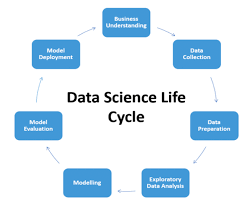
\includegraphics[width=8cm]{ds_cycle}
%         \caption{Data Science Cycle}
%         \label{fig:data science}
% \end{figure}



\clearpage
\section{Business-Intelligence-Systeme}

Was sind Business-Intelligence-Löungen?\\
%Wo kommen Buisiness-Intelligence-Lösungen zum Einsatz zum Einsatz?
Es gibt eine Vielzahl kommerzieller Lösungen für den Bibliotheksbereich, die auf Business-Intelligence-Software basieren.
Zu nennen wären \textit{AlmaAnalytics} für das Next-Generation-Library-System \textit{Alma} von \textit{ExLibris}\footnote{\url{https://www.exlibrisgroup.com/products/alma-library-services-platform/alma-analytics}
Stand: 26.05.2020}, \textit{BibControl} von \textit{OCLC}\footnote{\url{https://www.oclc.org/de/bibcontrol.html} Stand: 26.05.2020},
\textit{CollectionHq} von \textit{Baker \& Taylor}\footnote{\url{https://www.collectionhq.com/} Stand: 26.05.2020} oder \textit{Libinsight} von \textit{SpringShare}\footnote{\url{https://springshare.com/libinsight/} Stand: 26.05.2020}.
Darüber hinaus gibt es Business-Intelligence-Applikationen, die von
Bibliotheken für Reporting, Datenanalyse und Datenvisualisierung adaptiert werden,
wie zum Beispiel \textit{Tableau} von der Firma \textit{Tableau Software} oder
\textit{Crystal Reports} von \textit{SAP}.
Diese Applikationen sind entweder
an bestimmte Bibliothekssysteme zurückgebunden, limitiert in ihren
Funktionen\cite{golas_statistische_2018} oder zu generisch.
Überdies wird sowohl von \textit{HeBis} bzw. von der
Lokal-Bibliothekssystembetreuung als auch von der \textit{mpdl} keine Applikation
in dieser Richtung angeboten.
Ebenso ist ungewiss, wann die Ablösung des schon betagten \textit{CBS/LBS} hin zu
einem neuen Next-Generation-Library-System im \textit{HeBis-Verbund} stattfinden wird und ob
es ein Modul zur statistischen Datenerhebung liefern wird.
